\section{Luthfi Muhammad Nabil (1174035)}
\subsection{Membaca File PYSHP}
\begin{enumerate}
    \item Nomor 1
    \lstinputlisting{src/1/1174035/tugas3/soal1_1174035.py}
    \begin{figure}[H]
		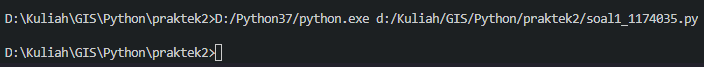
\includegraphics[width=6cm]{figures/1174035/tugas3/soal1_result.png}
		\centering
		\caption{Nomor 1}
	\end{figure}
    \item Nomor 2
    \lstinputlisting{src/1/1174035/tugas3/soal2_1174035.py}
    \begin{figure}[H]
		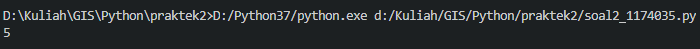
\includegraphics[width=6cm]{figures/1174035/tugas3/soal2_result.png}
		\centering
		\caption{Nomor 2}
    \end{figure}
    \item Nomor 3
    \lstinputlisting{src/1/1174035/tugas3/soal3_1174035.py}
    \begin{figure}[H]
		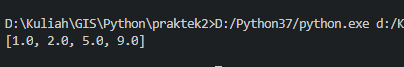
\includegraphics[width=6cm]{figures/1174035/tugas3/soal3_result.png}
		\centering
		\caption{Nomor 3}
    \end{figure}
    \item Nomor 4
    \lstinputlisting{src/1/1174035/tugas3/soal4_1174035.py}
    \begin{figure}[H]
		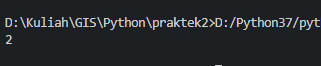
\includegraphics[width=6cm]{figures/1174035/tugas3/soal4_result.png}
		\centering
		\caption{Nomor 4}
    \end{figure}
    \item Nomor 5
    \lstinputlisting{src/1/1174035/tugas3/soal5_1174035.py}
    \begin{figure}[H]
		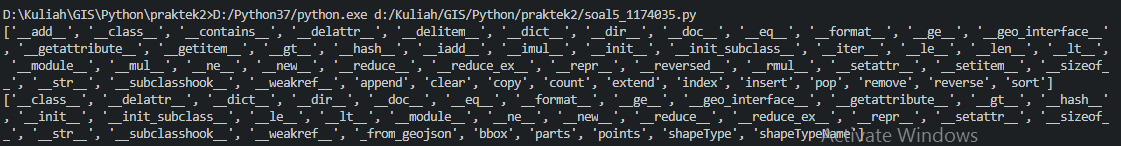
\includegraphics[width=6cm]{figures/1174035/tugas3/soal5_result.png}
		\centering
		\caption{Nomor 5}
    \end{figure}
    \item Nomor 6
    \lstinputlisting{src/1/1174035/tugas3/soal6_1174035.py}
    \begin{figure}[H]
		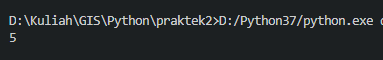
\includegraphics[width=6cm]{figures/1174035/tugas3/soal6_result.png}
		\centering
		\caption{Nomor 6}
    \end{figure}
    \item Nomor 7
    \lstinputlisting{src/1/1174035/tugas3/soal7_1174035.py}
    \begin{figure}[H]
		
\includegraphics[width=6cm]{figures/1174035/tugas3/soal7_result.png}
		\centering
		\caption{Nomor 7}
    \end{figure}
    \item Nomor 8
    \lstinputlisting{src/1/1174035/tugas3/soal8_1174035.py}
    \begin{figure}[H]
		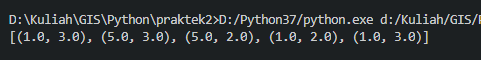
\includegraphics[width=6cm]{figures/1174035/tugas3/soal8_result.png}
		\centering
		\caption{Nomor 8}
    \end{figure}
    \item Nomor 9
    \lstinputlisting{src/1/1174035/tugas3/soal9_1174035.py}
    \begin{figure}[H]
		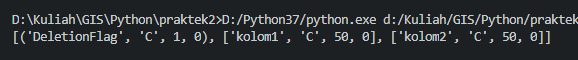
\includegraphics[width=6cm]{figures/1174035/tugas3/soal9_result.png}
		\centering
		\caption{Nomor 9}
    \end{figure}
    \item Nomor 10
    \lstinputlisting{src/1/1174035/tugas3/soal10_1174035.py}
    \begin{figure}[H]
		
\includegraphics[width=6cm]{figures/1174035/tugas3/soal10_result.png}
		\centering
		\caption{Nomor 10}
    \end{figure}
    \item Nomor 11
    \lstinputlisting{src/1/1174035/tugas3/soal11_1174035.py}
    \begin{figure}[H]
		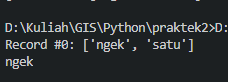
\includegraphics[width=6cm]{figures/1174035/tugas3/soal11_result.png}
		\centering
		\caption{Nomor 11}
	\end{figure}
\end{enumerate}
\subsection{Link Youtube}
\href{https://youtu.be/8i37HQsiDBg}{Praktek GIS}